
%
%  $Description: Author guidelines and sample document in LaTeX 2.09$
%
%  $Author: Gediminas Mazrimas $
%  $Date: 1995/09/15 15:20:59 $
%  $Revision: 1.4 $
%

\documentclass[times, 10pt,twocolumn]{article}
\usepackage{latex8}
\usepackage{times}

% Images includes
\usepackage{graphicx}
\usepackage{float}

%\documentstyle[times,art10,twocolumn,latex8]{article}

%-------------------------------------------------------------------------
% take the % away on next line to produce the final camera-ready version
\pagestyle{empty}

%-------------------------------------------------------------------------
\begin{document}

\title{Animating human model in OpenGL using data from Vicon system}

\author{Gediminas Mazrimas\\
Aalborg University Copenhagen\\ Computer Vision and Graphics\\g.mazrimas@gmail.com
\and
Algirdas Beinaravicius\\
Aalborg University Copenhagen\\ Computer Vision and Graphics\\algirdux@gmail.com
}

\maketitle
\thispagestyle{empty}

\begin{abstract}
   This paper explains how to animate 3D human model in OpenGL,
   avoiding most common problems, that occurs while dealing with
   various human body rigid parts transformations.
   The animation is associated with real person movements,
   while using data from Vicon motion capture system.
   Animating is made in lowest programming C++ OpenGL level.
   \\\\
   \textbf{Keywords:} Human animation, Vicon motion capture system, OpenGL, C++, Linear Blend Skinning
\end{abstract}



%-------------------------------------------------------------------------
\Section{Introduction}

Our animation focuses on the most common and partly simple human
body animation technique, that uses joints to animate human model. The joint structure,
given their position and orientation, can be thought as being human body skeleton.
The skin shape is associated to the joints, where as it's a 3D polygon mesh
and it's the only thing that is displayed for the end-user.
Due to very fast computation speeds, this technique is the most popular
in animation production. On the other hand, using simple shape blending technique
to deal with complex human body rigid parts transformations, there are
various skin deformation problems. Typical ones are collapsing elbow, candy-wrapper joint
when the arm turns 180 degrees, intersection between two adjacent bones (links) around a joint.
Also such a technique don't consider many very complicated and detail human body deformations,
for example dealing with muscles (stretch or bulge).

%-------------------------------------------------------------------------
\SubSection{Previous works}

What we've read and what was written there. References.
[Linear blend skinning, for deformation problems, data formats]

%-------------------------------------------------------------------------
\SubSection{Overview}

What is represented in further sections?

%-------------------------------------------------------------------------
\Section{Linear blend skinning}

Linear blend skinning technique is widely used for interactive applications.
It goes by many different names, such as Skeleton Subspace Deformation or SSD or smooth skinning" in Maya.

The linear blend skinning algorithm works by first placing a hierarchical
skeleton inside a static model mesh of a character in
some neutral pose (usually in the da Vinci posture or so called "dress pose").
Then, each vertex is assigned a set of influencing joints and a
blending weight for each influence. Computing the deformation in
some pose involves rigidly transforming each dress pose vertex by
all of its influencing joints. Then the blending weights are used to
combine these rigidly transformed positions.

The deformed vertex position, $ \overline{\textbf{v}} $ is
\begin{center}
$ \overline{\textbf{v}} = \displaystyle\sum_{i=1}^n\emph{w}_{i}M_{i}D_{i}^{-1}\textbf{v}_{d} $
\end{center}
where $w_{i}$ are the influence weights, $v_{d}$ is the dress-pose location of a
particular vertex \textbf{v}, $\emph{M}_{i}$ is the transformation matrix associated with
the $\emph{i}$th influence, and $D_{i}^{-1}$ is the inverse of the dress-pose matrix
associated with the $\emph{i}$th influence. Taken together, $D_{i}^{-1}\textbf{v}_{d}$ represents
the location of \textbf{v$_{d}$} in the local coordinate frame of the $\emph{i}$th influence.

\begin{figure}[H]
  \centering
  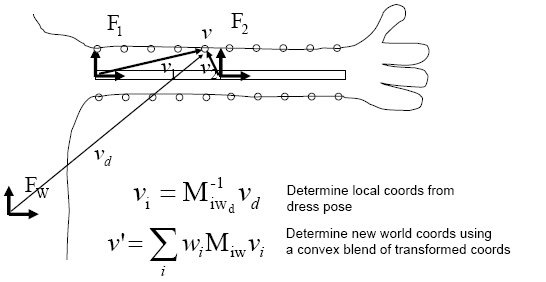
\includegraphics[width=93mm]{images/hand.jpg}
\end{figure}

Linear blend skinning though has two primary failings.
First, the method is incapable of expressing complex deformations.
Artifacts such as the "candy-wrapper", collapse effect on wrists and
collapsing around bending joints as shown appear. They
occur because vertices are transformed by linearly interpolated matrices.
If the interpolated matrices are dissimilar as in a rotation of
nearly 180 degrees, the interpolated transformation is degenerate,
so the geometry must collapse.
Second, authoring linear blend skins is difficult and frustrating for users.

Despite its failings, this skinning algorithm is very fast and
widely supported by commercial applications so it remains popular
especially in games and virtual environments.

%-------------------------------------------------------------------------
\Section{Motion capture}

Motion capture (\emph{mocap}) is sampling and recording motion of humans, animals, and inanimate
objects as 3D data. The data can be used to study motion or to animate 3D computer models.
During the motion capture process not only the capturing stage using \emph{mocap} equipment
is very important, as equally important are the preparation and post processing processes.
The whole system must be well calibrated, adjusted and set up, furthermore, after capturing
data needs to be cleaned, edited, and applied to a 3D model.

%-------------------------------------------------------------------------
\SubSection{Vicon MX motion capture system}

Vicon MX motion capture system is a passive optical system that uses markers
coated with a retroreflective material to reflect light back that is generated near the cameras lens.
The camera's threshold can be adjusted so only the bright reflective markers will be sampled, ignoring skin and fabric.

An object with markers attached at known positions is used to calibrate the cameras and obtain their positions and the lens distortion of each camera is measured. Providing two calibrated cameras see a marker, a 3 dimensional fix can be obtained.

Our system used for this project mainly consists of:

\begin{itemize}
\item 8 Vicon MX3+ cameras, fitted with sensitive solid-state
sensors, with stringent checks for linearity, sensitivity, and absence of jitter.
Each MX camera is programmed with firmware to control its operation
and enable it to perform its own onboard grayscale processing.
Cameras and their relevant characteristics are recognized immediately when they are plugged in to Vicon MX system.

\item MX Ultranet, that supplies power, synchronization, and
communications for all eight connected MX cameras. Only MX Ultranet is connected to the Host PC
and routes all communication to and from the host PC, and timing/synchronization signals to and from the
MX cameras connected to it.

\item Host PC, with seperate Ethernet port (preferably Gigabit ethernet card) to enable communications between
the Vicon software installed on this \emph{host pc} (in our case \emph{Vicon IQ 2.5}) and \emph{MX Ultranet}.
No other special requirements for Host PC, but processor and memory are vital for being able to achieve better results. Our \emph{host pc} had 2.49GB of RAM and 1.60GHz Intel Xeon 8 core processor.
\emph{Vicon IQ} software on a \emph{host pc} is used to collect
and process the raw video data. It takes the two-dimensional data from each
camera, combining it with calibration data to reconstruct the equivalent digital
motion in three dimensions. This can be viewed as a virtual
three-dimensional motion. After this reconstruction the data may be passed to
other applications.
\end{itemize}

\begin{figure}[H]
  \centering
  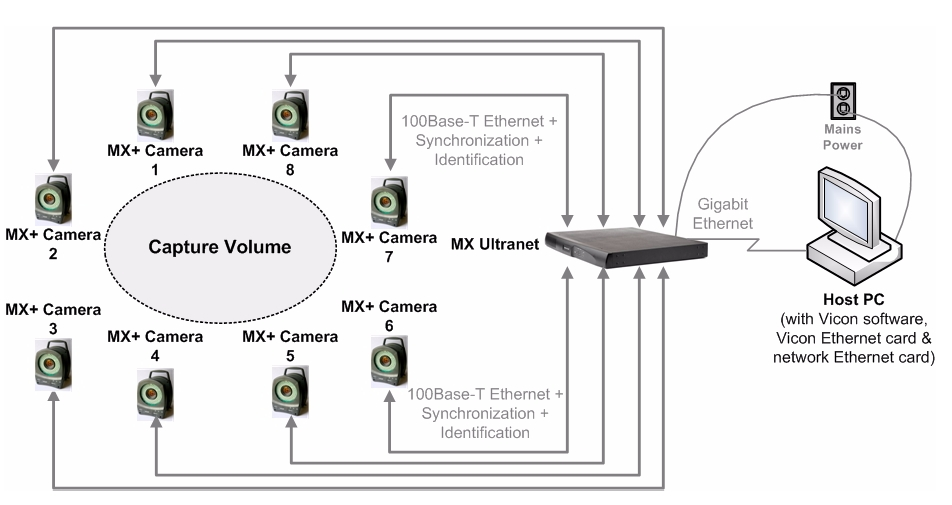
\includegraphics[width=98mm]{images/vicon_mx_basic.jpg}
\end{figure}

%-------------------------------------------------------------------------
\SubSection{System preparations}

Vicon motion capture system high-resolution cameras are situated in a circle,
above the maximum height of any marker that would be captured,
that forms a motion capture space. Then the capture volume is created.
The capture volume is three-dimensional, but in practice is more readily viewed
by its boundaries marked out on the floor. This gives you a guide for the
positioning of the cameras, and your subjects a guide as to where they
can move. The area should be as central to your capture space as possible
to maximize the volume you are able to capture.
Initially you are looking to see whether the camera is positioned and oriented
for the maximum view. Then every single camera can be adjusted separately
by changing software settings, to achieve best result.

After setting up cameras, the vital thing is system calibration.
It allows the software to calculate the relative location and
orientation of all the cameras. When your movements have been recorded the
reconstruction process uses these measurements to calculate the accurate
movements of the markers through space.

This is done by static and dynamic calibrations:

\begin{itemize}
\item Static calibration - calculates the origin or centre of the capture volume and determines the
orientation of the 3D Workspace.
\item Dynamic calibration - involves movement/waving of a calibration wand throughout the whole volume and
allows the system to calculate the relative positions and orientations of the
cameras. It also linearizes the cameras.
\end{itemize}

%-------------------------------------------------------------------------
\SubSection{Capturing data}

First step in capturing phase is placing all the reflective markers on special suit.
To correctly place them, the skeleton template must be selected that will be used for animation,
as it describes the bone structures, how many markers to use, and how those markers relate to the bone structure.

\begin{figure}[H]
  \centering
  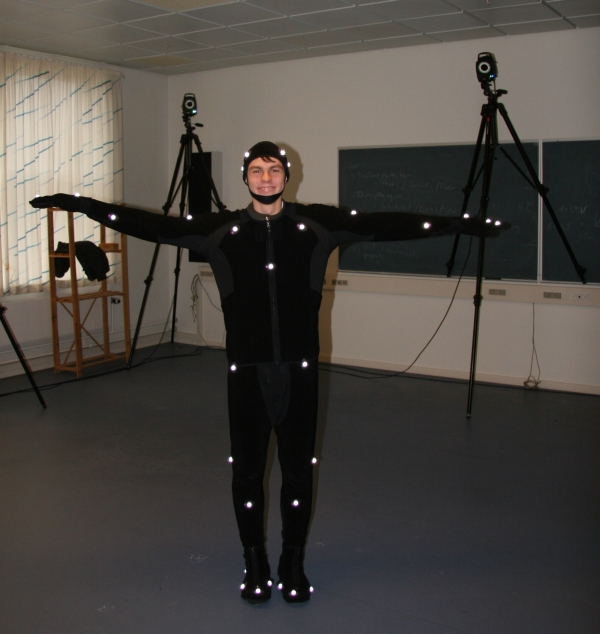
\includegraphics[width=70mm]{images/vicon_me.jpg}
\end{figure}

To start capturing, motion capture subject should stand in the middle of the circle in the capture are,
with his back straight, arms straight out with palms facing down, and feet forwards.
This is called a T-pose, and every capture session should begin and end every in it.

After capturing motion data, in order to proceed further, post-processing must be done.
It involves labeling/matching each marker from motion data to our used skeleton template.
Then special pipelines to automate many processes, for example match labeled markers in all the frames.
After all of that, manual calibration is also required, as there often occur some mismatches.

\begin{figure}[H]
  \centering
  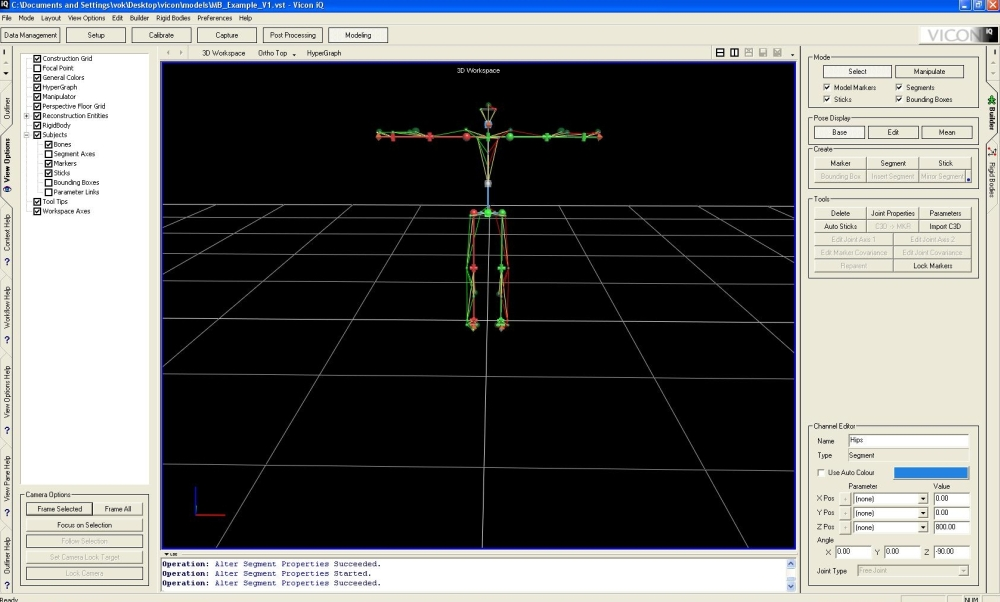
\includegraphics[width=90mm]{images/vicon.jpg}
\end{figure}

How we assign (label) captured data to a Vicon model. How Vicon model looks like
(available joints, their connections, connections to costume sensors).


%-------------------------------------------------------------------------
\Section{Motion data}

There are various \emph{motion data} storing formats, that mostly depend on what kind of program they
are being used on. Our aim on this project, considering motion data, was to select
the most appropriate data format. After reviewing some examples, the decision was made,
that the best choice for our model animation would be using \emph{BVH} motion data format.
But because our motion capture is being done using Vicon IQ software,
that's not able to directly export data to BVH file format, at first we had to work with Vicons' C3D
and then convert it to BVH.

%-------------------------------------------------------------------------
\SubSection{Description of Vicon C3D format}

This section is meant to give just a brief introduction to the C3D file format, describing it in an abstract way. A reference to a detailed manual, describing the format, is given in the reference part of this document.

The C3D (Coordinate 3D) file format is a binary data file format originally developed for the AMASS photogrammetry software system, capable of storing 3D data as well as analog data together with all associated parameters for a single measurement trial. Since only the 3D data is of importance, we will not consider analog data in this document. The main advantage of C3D format over other motion capture data formats is that it is able to encapsulate the motion data as well as parameters, describing the  motion data, in a single file. Apart from that, C3D is freely licensed and well documented.

Being a binary file, the C3D file consists of a number of 512-byte blocks. Logically C3D format can be divided into 3 basic sections, each having one or more 512-byte blocks:

    Header section is the first section of a file. The main purpose of this section is holding a pointer to the start of parameters section. Other parts of this section, is of no particular importance, as usually it consists data, copied from parameters section.

    The parameters section usually starts at block number 2, although this is not fixed and should not be assumed to be the case for every C3D file. This section contains information about the 3D data stored in the file. The section is extensible, meaning that user can define it's own parameters without  violating the format specification.

    Data section containing the 3D point coordinates is usually located after the parameters section. This section simply contains sequential frames data. In the case of 3D points (the data is X, Y and Z coordinates).

During the workflow of our project, the animation data, produced by the Vicon motion capturing system, was encoded in C3D file format. The data, provided by the C3D file, contains only the positions of skeleton joints at each frame, what is not sufficient to correctly animate the character. So the C3D animation data file was imported to Motion Builder, where the inverse kinematics technique was applied to provide us with BVH format file.  The BVH format file is another motion capturing data format, where the rotation data of each joint is being already calculated.


%-------------------------------------------------------------------------
\SubSection{Description of Biovision BVH format}

The BVH format is an updated version of BioVision�s BVA data format, with the addition of a
hierarchical data structure representing the bones of the skeleton.
The BVH file is an ASCII file and consists of two parts.

First section (\emph{hierarchy}) is for storing hierarchy and initial pose of the skeleton,
basically joint-to-joint connections and offsets.
While as second section (\emph{motion}) describes the channel motion data for each frame,
that is describes the movement of individual joints.

The \emph{hierarchy} section starts with \emph{root} joint and contains the definition of a joint hierarchy within nested braces like source code written in the C programming language.
Each joint in a \emph{hierarchy} has an \emph{offset} field and a \emph{channels} field.
The \emph{offset} field stores initial \emph{offset} values for each joint with respect to its parent joint.
\emph{channels} field defines which �channels� of transformation (translation and/or rotation) exist for the joint in
the \emph{motion} data section of the file. The \emph{channels} field also defines the order of transformation. A
\emph{channel} is either x-, y-, or z-translation or local x-, y-, or z-rotation. All the segments are assumed
to be rigid and scaling is not available.
The \emph{end site} field is also available in order to determine body segment end.

In the \emph{motion} section the total number of frames in the animation and the frame
speed in frames-per-second is defined. Every next row then contains data values for all \emph{channels} which were specified in the \emph{hierarchy} section.
The listing order of \emph{motion} values in each row in is assumed to match their listed order from the \emph{hierarchy} section (top down).

There are few drawbacks of the BVH format. One is that it lacks a full definition of the initial pose. Another
drawback is that the format has only translational offsets of children segments from their parents. No
rotational offset can be defined. Moreover, the BVH format is often implemented differently in different
applications, that is, one BVH format that works well in one application may not be interpreted
in another. All the same the format is very flexible and it is relatively easy to edit BVH files.

\textbf{[Give more details later about exact structure of our model (like example)]}

%-------------------------------------------------------------------------
\SubSection{Processing captured data}
Why do we need to convert C3D data to BVH?
What's good and bad about them? (C3d would be faster,
but it's binary, so not a human readable,
also BVH gives us rotations and have good structure,
that is much easier to implement in our C++ program).
How do we do it using Motion builder?


While C3D gives us our marker coordinates from motion capture system,
by labeling these markers at first in Vicon system and then importing them
in Motion builder, in BVH then we get rotations and translations not for those
markers, but for human body model joints.

\begin{figure}[H]
  \centering
  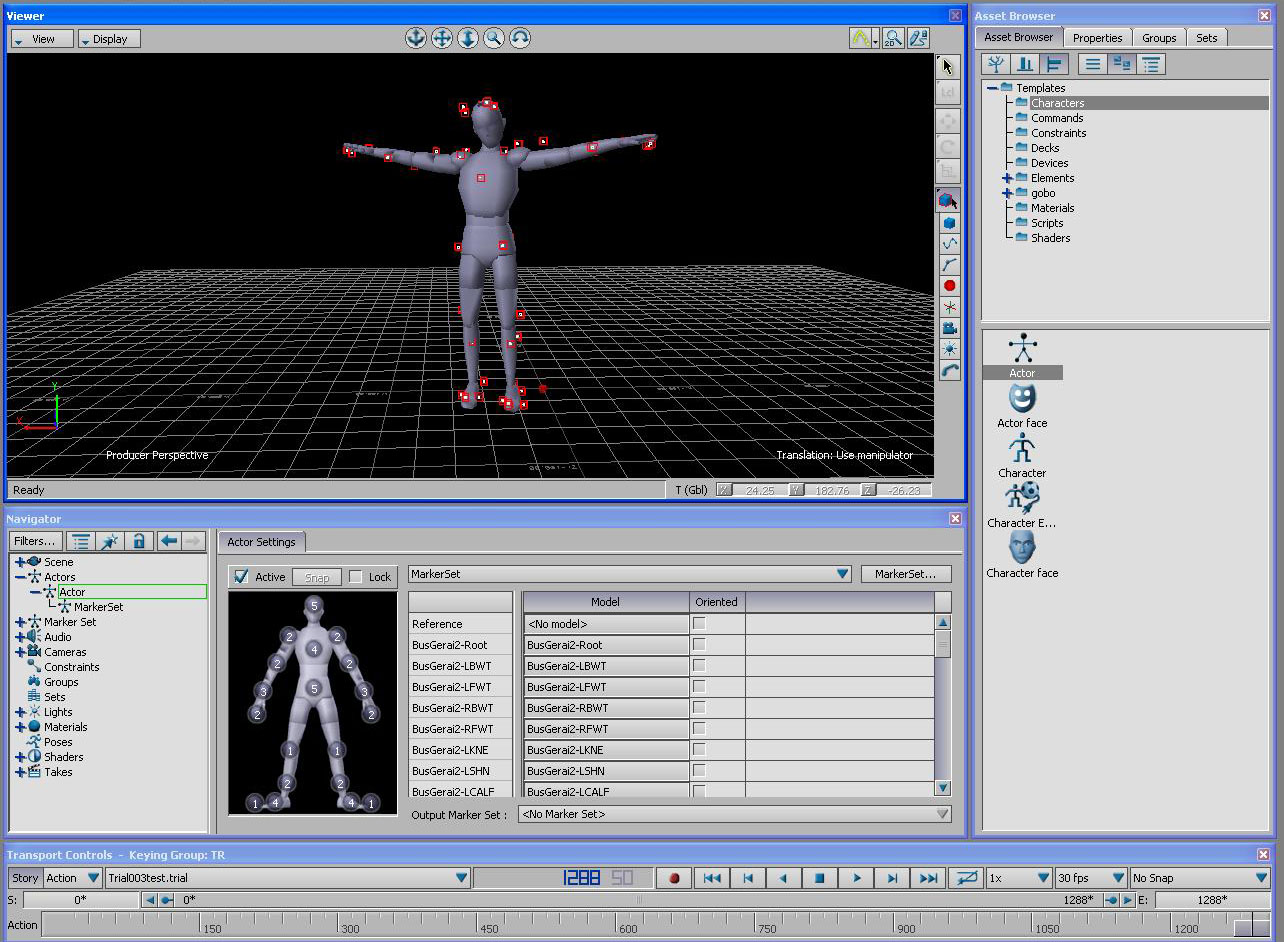
\includegraphics[width=90mm]{images/mb.jpg}
\end{figure}

[Here goes how we interpret BVH data]


%-------------------------------------------------------------------------
\Section{Human body mesh model}

What do we use for our animation?

%-------------------------------------------------------------------------
\SubSection{Mesh model preparations in Maya}

What Mesh model in Maya do we use?
How do we prepare it, that it would be suitable for out program?
How we cut mesh to different body parts, export to .obj format files.

%-------------------------------------------------------------------------
\SubSection{Mesh model file format used in animation}

Why do we use .obj file format? How does it look like?


%-------------------------------------------------------------------------
\SubSection{Description of OBJ format}

OBJ is a geometry definition file format, first developed by Wavefront technologies. The file format is open and has been adopted by most of 3D graphics application vendors. It can be imported/exported from most of 3D modeling tools such as Autodesk's Maya, 3ds Max, Newtek's Lightwave, Blender, etc.  This section of the document provides a  thorough explanation of the most important parts of an object file, with more details provided in the reference page.

An object file can be stored in ASCII (using the ".obj" file extension) or in binary format (using the .MOD extension). The binary format is proprietary and undocumented, so only the ASCII format is described here.

The OBJ file format supports lines, polygons, and free-form curves and surfaces. Lines and polygons are described in terms of their points, while curves and surfaces are defined with control points and other information depending on the type of curve. Since, in our project, lines and polygons were sufficient to represent the model appropriately, only the parameters, concerning, these entities are described below.

The OBJ file is composed of lines of text, each of them starting with a token, which describes the type of the entity being  recorded in that line. Below are listed various tokens, which were of importance in our project:

\begin{itemize}
\item "\#" - a comment line. Lines, starting with "\#" token, are simply skipped by OBJ file readers. For example "\# this is a comment".
\item "g" - a group line. Lines, starting with "g" (group) token, determine the start of a group. "g" token is followed by the group name. For example $"g left_arm"$. In our project each group name corresponded to some body part, described by vertices, textures, normals and polygons.
\item "v" - a vertex line. Lines, starting with "v" (vertex) token, provide the information, concerning vertices. This token is followed by x, y and z coordinates of the vertex. For example "v -0.756447 0.702621 0.047024" is a vertex with coordinates (-0.756447, 0.702621, 0.047024).
\item "vt" - a texture line. Lines, starting with "vt" (vertex texture) token, are recorded with information, concerning textures. "vt" token is followed by x, y and z coordinates of the texture, although only the x and y coordinates are of importance (z coordinate is 0.0). For example "vt 0.487840 0.942165 0.000000".
\item "vn" - a vertex normal line. Lines, starting with "vn" (vertex normal) token, contain information, concerning the normal of a vertex. "vn" token is followed by x, y and z coordinates of the normal. For example "vn 0.149280 -0.186998 -0.240511".
\item "f" - a line, describing face. Lines, starting with "f" (face) token, provide the information, concerning polygons. "f" token is followed by a number of triplets, which is equal to the number of vertices, the polygon has. Each triplet is of a form "int/int/int", where the first "int" is a vertex position in the file, the second "int" is "texture" position in the file and the third "int" is a normal position in the file. For example "f 6/9/6 2/5/2 1/1/1" is a triangle polygon, with vertices 6, 2 and 1, textures 9, 5 and 1 and normals 6, 2 and 1.
\end{itemize}

The above described tokens were of importance in our project, but they are not the only ones that OBJ format allows. The OBJ format specification is much broader and covers such abilities as surface encoding, connectivity between free-form surfaces, rendering attributes. The OBJ specification can be found in the document's reference page.



%-------------------------------------------------------------------------
\Section{Animating human body}

Explain how we load human model, exported from Maya to .obj file.
How we create natural primary human pose, assign meshes to joints and so on.

%-------------------------------------------------------------------------
\SubSection{Loading human body model in OpenGL}

How we load human body to OpenGL. How we import mesh from obj files.
Joint creation. Joint connection with meshes.

%-------------------------------------------------------------------------
\SubSection{Linear blend skinning relations}

How we adapted linear blend skinning to our animations.
Explain how our method using meshes assigned with joint rotations
is similar to linear blend skinning. How we automated all the things.


%-------------------------------------------------------------------------
\Section{Conclusion}
Conclusion

%-------------------------------------------------------------------------
\SubSection{Future work}
What could be implemented to improve this project?
Live streaming to our animating program (straight from cameras to animation in OpenGL);
other skin deformations


%-------------------------------------------------------------------------
\nocite{ex1,ex5,ex2,ex3,ex4,ex6}
\bibliographystyle{latex8}
\bibliography{latex8}

\end{document}

